\chapter{Metodología}
\label{ch:methodology}

\TODO{Esto lo saco del paper de modelling blablabla de lane execution. Lo pongo aquí porque lcreo que lo suyo es poner la metodologías entera aquí. Además el tema de instrumentación, los recorridos, etcétera esta bien que estén aquí englobados. Hay que tener cuidado de, si se pone una cronología, que sea cierta, es decir, primero lane execution, luego lane intention, ...}

Para entrenar, comparar y validar los diferentes modelos de aceptación de cambio de carril, se ha seguido el siguiente método. Se utiliza un vehículo instrumentado para registrar los datos de conducción, primero, para el reconocimiento de patrones de conducción para clasificar los controladores en dos subconjuntos y segundo, para la construcción de conjuntos de datos para el proceso de formación de modelos. En el segundo caso, un operador estará presente en el vehículo y le pedirá a los sujetos que realicen un cambio a la izquierda o a la derecha en diferentes situaciones (principalmente con y sin automóviles en el entorno) mientras se graban los datos. Esos eventos luego se registran como intención de cambio de carril porque los sujetos deben ejecutar el cambio de carril si es posible. De esta forma, garantizamos que cada ejecución de cambio de carril (o imposibilidad de ejecución) está directamente relacionada con una intención de cambio de carril.

Las secciones que siguen describen cómo se instrumenta el vehículo, y se obtienen datos, cómo se procesan a una representación adecuada para entrenar a los modelos y, finalmente, cómo se entrena a los modelos.

\section{Instrumentación del vehículo}

El vehiculo usado para el desarrollo de esta tesis es un Mitsubishi iMiEV (Figura~\ref{fig:instrumented-imiev}). Éste ha sido instrumentado con los siguientes dispositivos:

\begin{figure}
	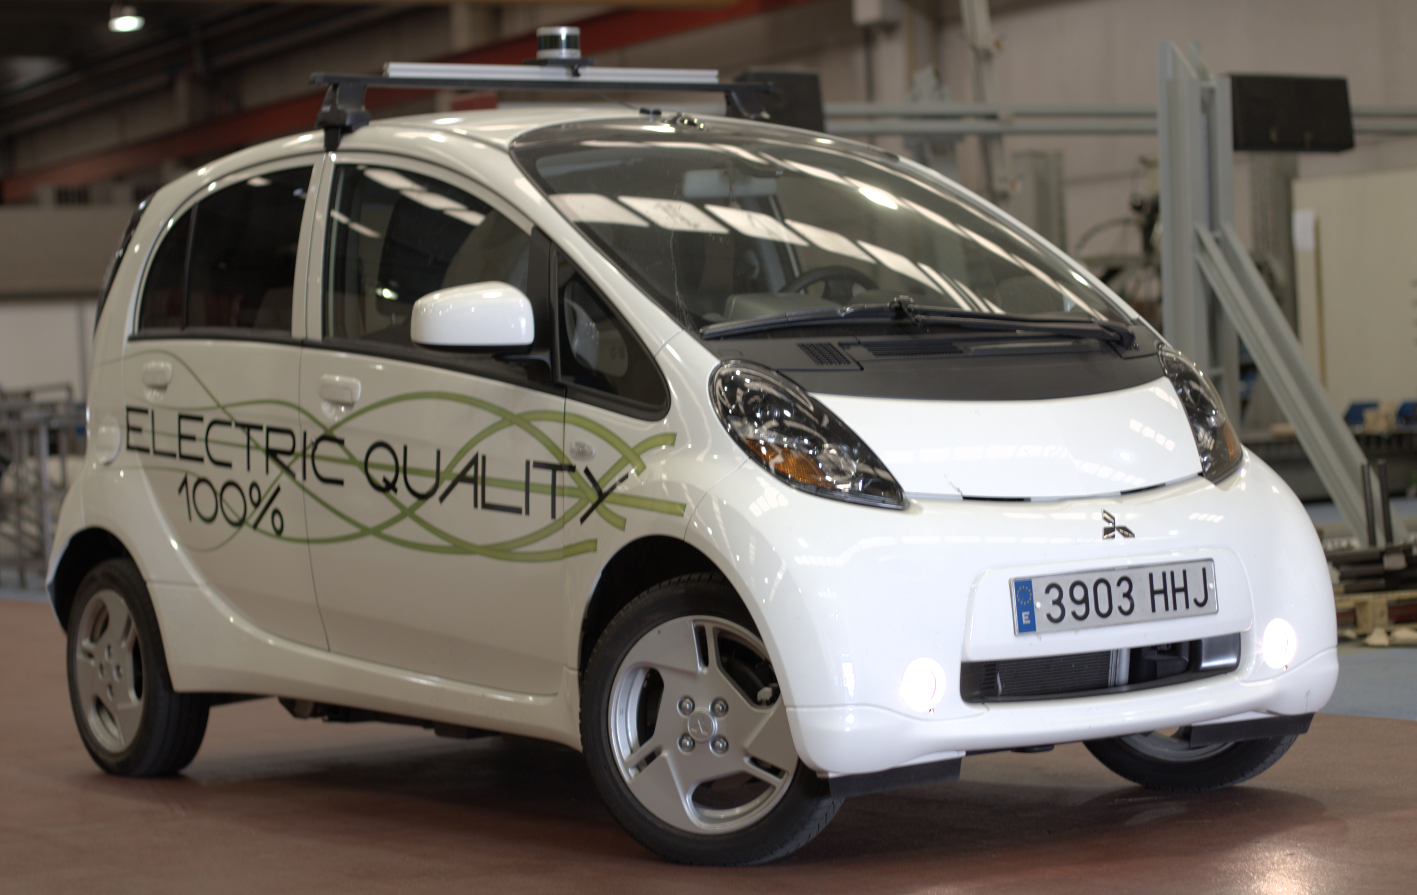
\includegraphics{instrumented-imiev}
	\caption{The instrumented Mitsubishi iMiEV.}
	\label{fig:instrumented-imiev}
\end{figure}

\begin{itemize}
	\item \textbf{LiDAR}. \TODO{explicación de qué es un LiDAR. Algo cortito del estilo mide la distancia a través la diferencia entre la emisión de pulsos de luz y su reflejo en un sensor. A lo mejor queda bien en un sidenote}. El usado es un Velodyne VLP-16, un LiDAR circular de 16 canales verticales separados 2º, dando un FOV (-15, 15) grados de apertura vertical). Este dispositivo se conecta a la máquina a través del puerto ethernet y se usa para la obtención de información del entorno del conductor. El LiDAR está situado en el techo del vehículo orientando los (0, 0) grados en al dirección y sentido de éste y con el plano horizontal paralelo al suelo.
	\item \textbf{Keyboard}. \TODO{No sé si ponerlo, pero al menos habría que mencionarlo, aquí o más adelante en el apartado específico de la ejecución de cambio de carril. A lo mejor se podría disfracar como un "gestionador de eventos" o algo así y poner un mando o unos botones de recreativa, que eso siempre queda bien.} Un teclado común conectado a través del puerto usb para funcionar como detector de eventos.
	\item \textbf{CAN Bus}. \TODO{Explicar qué es el CAN Bus, y si es necesario, un poquitín su funcionamiento (aunque sea en un sidenote, así queda todo más completito.)}. El BUS del vehículo se conecta a través del puerto USB al ordenador \TODO{a lo mejor hay que explicar un poco más la conexión, el tipo de cable y tal}. Es usado para la extracción de la interacción del conductor con el vehículo.
	\item \textbf{GPS Receiver}. \TODO{A lo mejor este no es necesario ponerlo. Yo creo que se podría decir que se usa para obtener una segunda medida de velocidad y aceleración, así como para la localización espacial de subconjuntos de datos interesantes para su estudio.}
\end{itemize}

Todos los dispositivos se conectan a un ordenador con sistema operativo Ubuntu GNU/Linux sobre Intel i7-6400U CPU con 8GB de memoria RAM. El esquema del vehículo instrumentado se detalla en la Figura~\ref{fig:instrumented-imiev-schema}.

\begin{figure}
	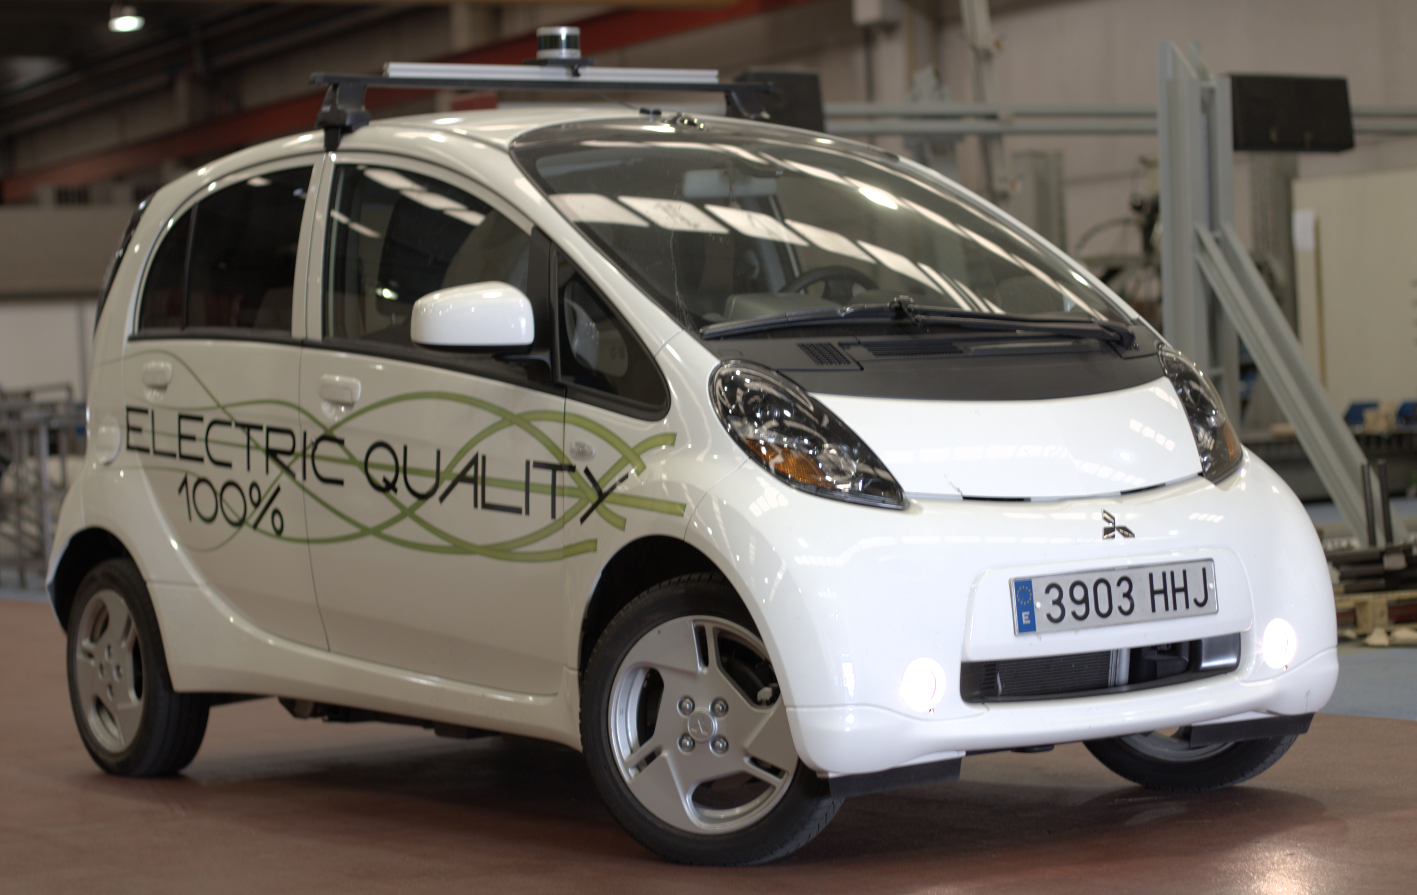
\includegraphics{instrumented-imiev-schema}
	\caption{The instrumented vehicle schema.}
	\label{fig:instrumented-imiev-schema}
\end{figure}

Todos los dispositivos han sido, o bien configurados para una captura a 10Hz de frecuencia, o bien remuestreados a ésta. La tabla~\ref{tbl:data-obtained-from-instrumented-vehicle} resume los datos recogidos y su dominio.

\begin{table}[t]
	\caption[Resúmen de información extraída del vehículo instrumentado][1.5em]{Valores capturados por el vehículo instrumentado y sus dominios. Los valores de 0, 1 y 2 se corresponden con los cambios de carril, siendo 0 cambio a la izquierda, 1 no cambio y 2 a la derecha.}
	\label{tbl:data-obtained-from-instrumented-vehicle}
	\begin{tabular}{lll}
		\toprule
		Variable & Descripción & Dominio \\
		\midrule
		LiDAR & Coordenadas de todos los puntos capturados por el dispositivo. & $[-200m, 200m] \subset \mathbb{R}$ \\
		\bottomrule
	\end{tabular}
\end{table}

\section{Perfiles de conducción}

Para tener suficiente información con la que trabajar, se han usado datos pertenecientes a conjuntos de conductores con diferentes perfiles de conducción. Todos los sujetos empleados en el experimento tiene el mismo rango de edad y género.

Tras obtener sus datos en rutas de prueba preliminares en entorno urbano, los sujetos se separaron en dos conjuntos de conductores con perfiles de conducción diferentes tal y como se describe en~\cite{DiazAlvarez2014}. Los sujetos cuyos datos eran difícilmente caracterizables no fueron incluidos en ninguno de los conjuntos.

Los parámetros usados para la clasificación corresponden al promedio y las varianzas de los 7 indicadores (uno para la velocidad, dos para la aceleración y cuatro para los tirones) para un total de 14 indicadores. Los valores se han normalizado para resaltar la diferencia entre ambos perfiles de la siguiente manera:

\begin{itemize}
	\item \textbf{Velocidad}. Media normalizada en el intervalo $[0, 20]$ y varianza en el intervalo $[0, 400]$.
	\item \textbf{Aceleración} y \textbf{jerk}. Media y varianza en el intervalo $[0, 2]$.
\end{itemize}

Los valores brutos se representan en la Tabla~\ref{tbl:raw-indicators-from-drivers-profiles}. Sus perfiles se han extraído de los datos de GPS y CAN Bus como se describe en [1]. La figura muestra el perfil normalizado para los datos de los dos subconjuntos de controladores (llamados Sm y Se).

\begin{table}
	\caption[Indicadores de los datos extraídos de cada perfil]{Indicadores extraídos a partir de los datos de cada perfil de conducción.}
	\label{tbl:raw-indicators-from-drivers-profiles}
	\begin{tabular}{@{}lllll@{}}
		\toprule
		\multirow{2}{*}{Indicador} & \multicolumn{2}{c}{$S_m$} & \multicolumn{2}{c}{$S\_e$} \\
		& $\mu$ & $\sigma$ & $\mu$ & $\sigma$ \\ \midrule
		Speed & 17.75 & 349.31 & 17.96 & 307.25 \\
		Negative acceleration (NA) & 1.91 & 4.44 & 1.52 & 1.91 \\
		Positive acceleration (PA) & 1.73 & 3.68 & 1.37 & 1.87 \\
		Starting movement jerk (SMJ) & 1.66 & 3.50 & 1.20 & 1.69 \\
		Cruising track jerk (CTJ) & 1.61 & 2.34 & 1.21 & 0.99 \\
		Starting brake jerk (SBJ) & 1.60 & 2.20 & 1.18 & 1.49 \\
		Ending brake jerk (EBJ) & 1.59 & 2.40 & 1.30 & 2.00 \\
		\bottomrule
	\end{tabular}
\end{table}

\begin{figure}
	\centering
	\subfloat[]{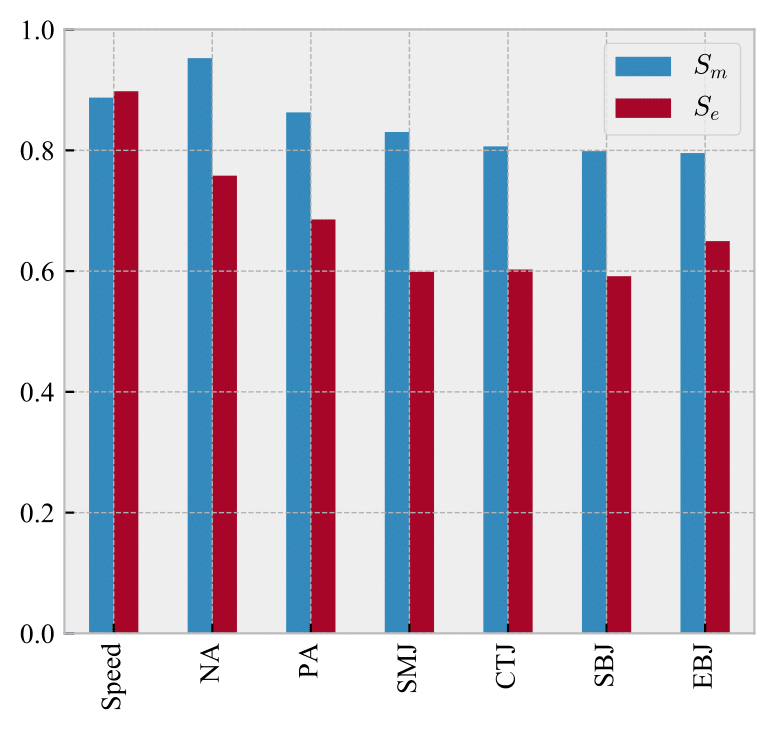
\includegraphics[width=.47\textwidth]{raw-indicators-from-drivers-profiles-a}}\qquad
	\subfloat[]{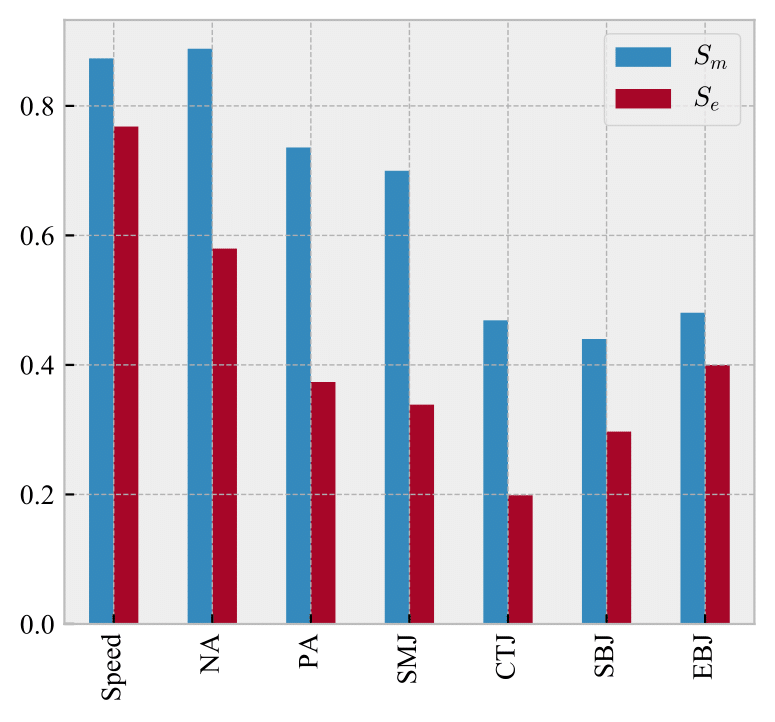
\includegraphics[width=.47\textwidth]{raw-indicators-from-drivers-profiles-b}}
	\caption{Comparación de indicadores entre los diferentes perfiles de conducción.}
	\label{fig:raw-indicators-from-drivers-profiles}
\end{figure}

\section{Routes}

Para la captura de datos se prepararon dos rutas, $R_1$ para utilizar los datos extraídos como datos de entrenamiento de los modelos y $R_2$ como datos para el proceso de validación de los mismos. La Figura~\ref{fig:proposed-routes} muestra los mapas para éstas. Ambas son rutas urbanas con una duración de aproximadamente 20 minutos, con tramos de uno y dos carriles, y en las que las velocidades máximas permitidas oscilan entre los 20 y los 50 \si{\kilo\metre\per\hour}. Fueron realizadas entre las 11:00am y las 12:00pm en días laborables, permitiendo una circulación con suficientes vehículos para conducir, pero sin demasiados como para impedir la circulación.

\begin{figure}
	\centering
	\subfloat[]{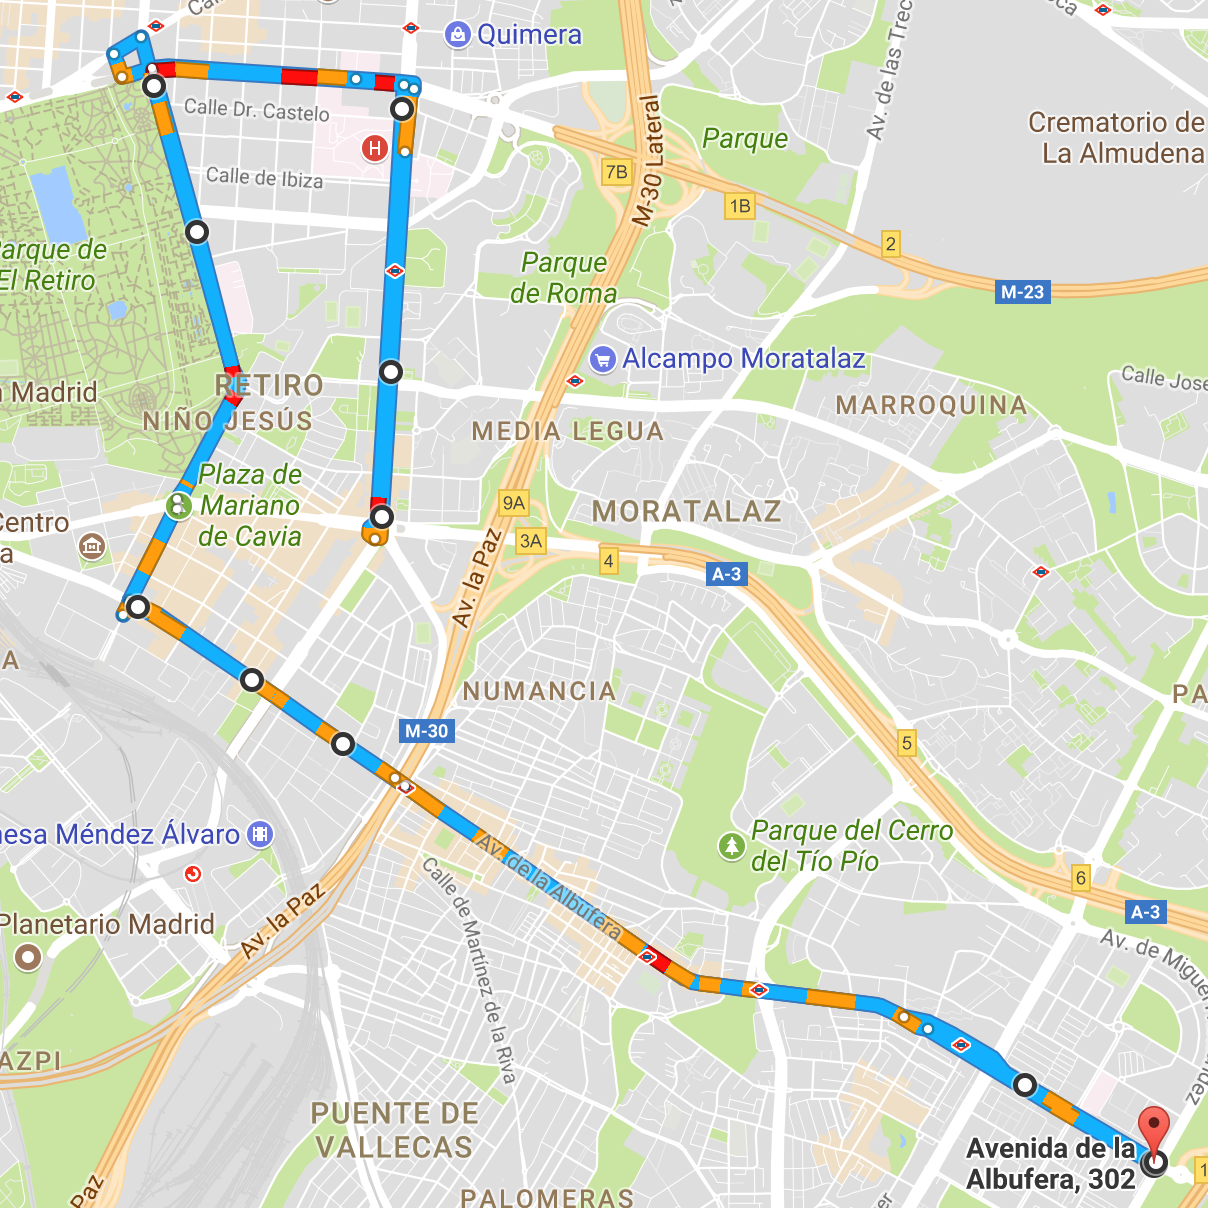
\includegraphics[width=.45\textwidth]{route-1}}\qquad
	\subfloat[]{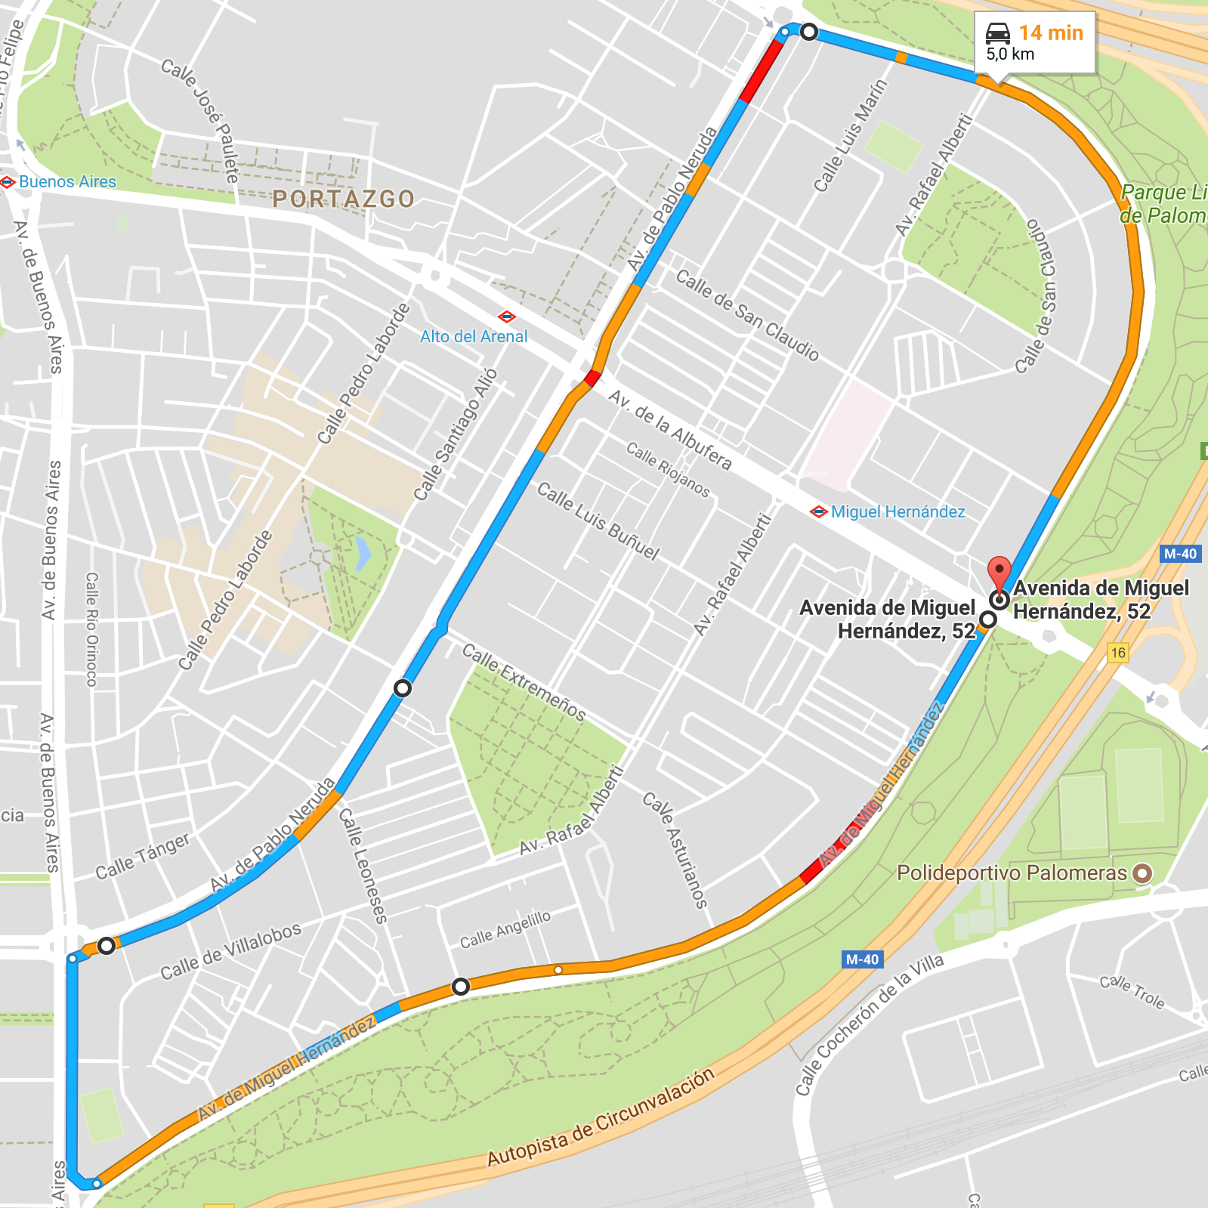
\includegraphics[width=.45\textwidth]{route-2}}
	\caption{Las dos rutas del experimento, (a) Ruta $R_1$ para entrenamiento y (b) Ruta $R_2$ para validación.}
	\label{fig:proposed-routes}
\end{figure}

Los sujetos realizaron la ruta primero para familiarizarse con el circuito. Posteriormente, las rutas fueron realizadas y los datos extraídos para el resto del proceso.

\section{Proceso de los datos}

Tras la captura, los datos fueron preprocesados antes de entrenar los modelos. Los datos de cada modelo fueron preprocesados de manera distinta, por lo que este proceso quedará descrito más adelante en las secciones dedicadas a éstos.
